\documentclass{book}
%book, article, report, beamer, uinwsskripsi

\usepackage[bahasa]{babel}
\usepackage{graphicx}

%\renewcommand{\chaptername}{BAB}

\begin{document}
\chapter{Pendahuluan}

\section{Latar Belakang}
tes gambar \ref{gb:kereta}

\begin{figure}[h]
\label{gb:kereta}
\centering
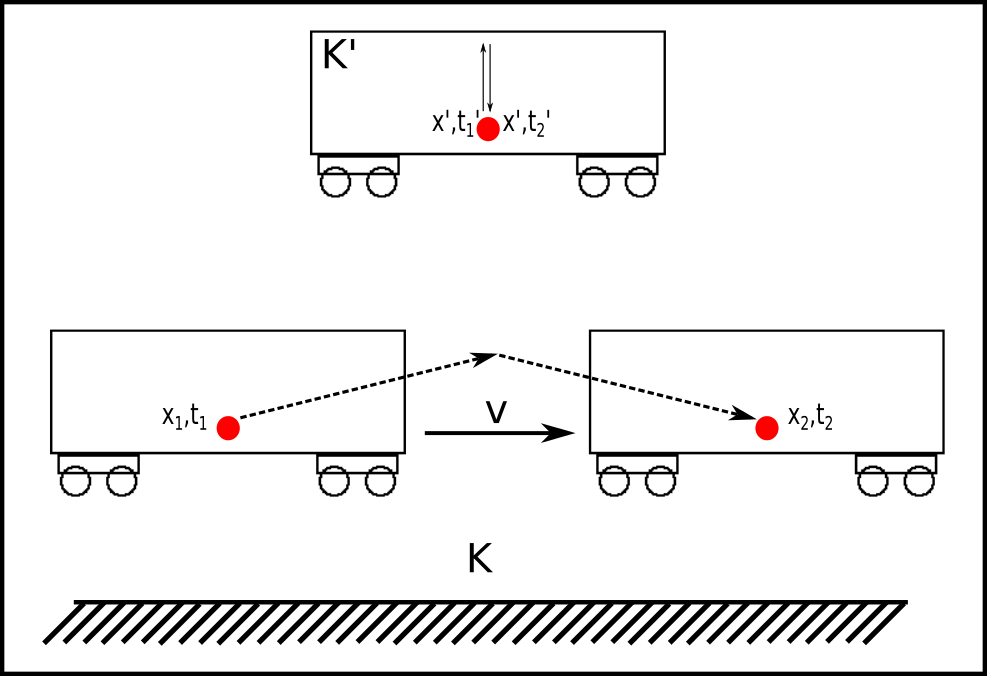
\includegraphics[width=5cm, height=5cm]{kereta.png}
\caption{Kereta}
\end{figure}

\begin{enumerate}
%\setcounter{enumi}{10}
\item Fisika
\item Kimia
\item Matematika
\end{enumerate}

\begin{itemize}
\item[a.] Fisika
\item Kimia
\item Matematika
\end{itemize}

\end{document}

% https://tableconvert.com/